\documentclass[man,floatsintext]{apa6}
\usepackage{lmodern}
\usepackage{amssymb,amsmath}
\usepackage{ifxetex,ifluatex}
\usepackage{fixltx2e} % provides \textsubscript
\ifnum 0\ifxetex 1\fi\ifluatex 1\fi=0 % if pdftex
  \usepackage[T1]{fontenc}
  \usepackage[utf8]{inputenc}
\else % if luatex or xelatex
  \ifxetex
    \usepackage{mathspec}
  \else
    \usepackage{fontspec}
  \fi
  \defaultfontfeatures{Ligatures=TeX,Scale=MatchLowercase}
\fi
% use upquote if available, for straight quotes in verbatim environments
\IfFileExists{upquote.sty}{\usepackage{upquote}}{}
% use microtype if available
\IfFileExists{microtype.sty}{%
\usepackage{microtype}
\UseMicrotypeSet[protrusion]{basicmath} % disable protrusion for tt fonts
}{}
\usepackage{hyperref}
\hypersetup{unicode=true,
            pdftitle={The title},
            pdfauthor={First Author~\& Second Author},
            pdfkeywords={keywords},
            pdfborder={0 0 0},
            breaklinks=true}
\urlstyle{same}  % don't use monospace font for urls
\usepackage{graphicx,grffile}
\makeatletter
\def\maxwidth{\ifdim\Gin@nat@width>\linewidth\linewidth\else\Gin@nat@width\fi}
\def\maxheight{\ifdim\Gin@nat@height>\textheight\textheight\else\Gin@nat@height\fi}
\makeatother
% Scale images if necessary, so that they will not overflow the page
% margins by default, and it is still possible to overwrite the defaults
% using explicit options in \includegraphics[width, height, ...]{}
\setkeys{Gin}{width=\maxwidth,height=\maxheight,keepaspectratio}
\IfFileExists{parskip.sty}{%
\usepackage{parskip}
}{% else
\setlength{\parindent}{0pt}
\setlength{\parskip}{6pt plus 2pt minus 1pt}
}
\setlength{\emergencystretch}{3em}  % prevent overfull lines
\providecommand{\tightlist}{%
  \setlength{\itemsep}{0pt}\setlength{\parskip}{0pt}}
\setcounter{secnumdepth}{0}
% Redefines (sub)paragraphs to behave more like sections
\ifx\paragraph\undefined\else
\let\oldparagraph\paragraph
\renewcommand{\paragraph}[1]{\oldparagraph{#1}\mbox{}}
\fi
\ifx\subparagraph\undefined\else
\let\oldsubparagraph\subparagraph
\renewcommand{\subparagraph}[1]{\oldsubparagraph{#1}\mbox{}}
\fi

%%% Use protect on footnotes to avoid problems with footnotes in titles
\let\rmarkdownfootnote\footnote%
\def\footnote{\protect\rmarkdownfootnote}


  \title{The title}
    \author{First Author\textsuperscript{1}~\& Second Author\textsuperscript{1,2}}
    \date{}
  
\shorttitle{Title}
\affiliation{
\vspace{0.5cm}
\textsuperscript{1} School 1\\\textsuperscript{2} Institute B}
\keywords{keywords\newline\indent Word count: X}
\usepackage{csquotes}
\usepackage{upgreek}
\captionsetup{font=singlespacing,justification=justified}

\usepackage{longtable}
\usepackage{lscape}
\usepackage{multirow}
\usepackage{tabularx}
\usepackage[flushleft]{threeparttable}
\usepackage{threeparttablex}

\newenvironment{lltable}{\begin{landscape}\begin{center}\begin{ThreePartTable}}{\end{ThreePartTable}\end{center}\end{landscape}}

\makeatletter
\newcommand\LastLTentrywidth{1em}
\newlength\longtablewidth
\setlength{\longtablewidth}{1in}
\newcommand{\getlongtablewidth}{\begingroup \ifcsname LT@\roman{LT@tables}\endcsname \global\longtablewidth=0pt \renewcommand{\LT@entry}[2]{\global\advance\longtablewidth by ##2\relax\gdef\LastLTentrywidth{##2}}\@nameuse{LT@\roman{LT@tables}} \fi \endgroup}


\DeclareDelayedFloatFlavor{ThreePartTable}{table}
\DeclareDelayedFloatFlavor{lltable}{table}
\DeclareDelayedFloatFlavor*{longtable}{table}
\makeatletter
\renewcommand{\efloat@iwrite}[1]{\immediate\expandafter\protected@write\csname efloat@post#1\endcsname{}}
\makeatother
\usepackage{lineno}

\linenumbers
\newcommand{\beginsupplement}{\setcounter{table}{0}  \renewcommand{\thetable}{S\arabic{table}} \setcounter{figure}{0} \renewcommand{\thefigure}{S\arabic{figure}}}

\authornote{

Correspondence concerning this article should be addressed to First
Author, Postal address. E-mail:
\href{mailto:my@email.com}{\nolinkurl{my@email.com}}}

\abstract{

}

\begin{document}
\maketitle

\hypertarget{introduction}{%
\section{Introduction}\label{introduction}}

Lorem ipsum dolor sit amet, consectetur adipiscing elit. Nullam a magna
ac lorem aliquet pellentesque et bibendum diam. Phasellus in lectus
malesuada, consequat arcu quis, dignissim massa. Donec laoreet egestas
leo, et tristique tortor cursus at. Aenean non molestie orci, sit amet
bibendum sem. Sed convallis vulputate tortor quis sagittis. Aliquam
placerat lacus at urna sodales, id facilisis libero fringilla. Quisque
ac orci id ex fermentum euismod. Pellentesque tempor, urna vel
sollicitudin mollis, purus ex ornare eros, sed suscipit orci enim sed
sem. Mauris quis purus ut purus congue tincidunt. Suspendisse potenti.
Maecenas mauris velit, imperdiet nec feugiat ut, eleifend a urna.
Vestibulum arcu lacus, suscipit eu tincidunt et, sodales eget lectus.
Donec sit amet accumsan est.

Vivamus ligula urna, scelerisque nec sem sit amet, condimentum pharetra
magna. Nullam tincidunt ipsum ut dolor rutrum, ac malesuada eros
blandit. Vestibulum consectetur ultricies lectus, quis cursus risus
fermentum sed. Proin non nunc eget sem commodo faucibus et sed ex. Ut in
orci lorem. Morbi vehicula, lorem vitae fermentum egestas, odio felis
rutrum nisi, nec mattis elit nisl vel libero. Vivamus facilisis nisi id
mauris lobortis, ut egestas massa tristique. Nam ac massa facilisis,
molestie arcu ut, finibus tellus.

Sed sagittis velit ac nisi egestas, a maximus lorem congue. Nulla
sodales laoreet tortor eleifend congue. Aliquam et felis vehicula,
condimentum mauris non, varius purus. Nunc ligula ex, volutpat interdum
interdum sed, porta ut eros. Duis molestie, turpis sed aliquam rhoncus,
orci dui lacinia mauris, ut feugiat mauris leo at enim. Mauris non
tortor eleifend, vulputate justo sit amet, ullamcorper risus. Vestibulum
in odio sed erat venenatis imperdiet ac at massa.

\hypertarget{materials-and-methods}{%
\section{Materials and Methods}\label{materials-and-methods}}

\hypertarget{data}{%
\subsection{Data}\label{data}}

\hypertarget{analyses}{%
\subsection{Analyses}\label{analyses}}

We used R for all analyses (R Core Team, 2018).

\hypertarget{results}{%
\section{Results}\label{results}}





\begin{figure}[!h]
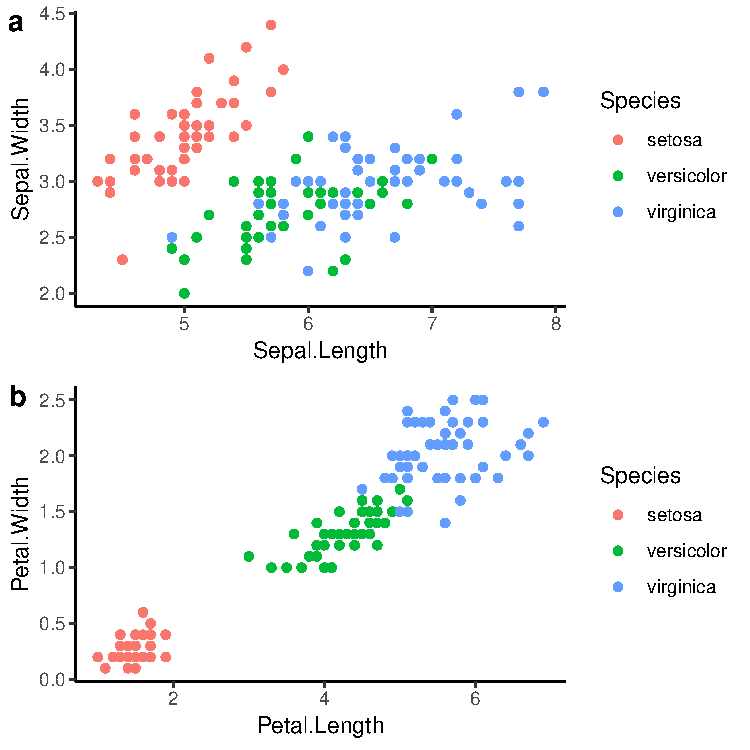
\includegraphics[width=\textwidth]{../Figures/iriscorrelationsplot} \caption{Sepals and petals in three \emph{Iris}
species. (a) Relationship between sepal length and width. (b)
Relatiopnship between petal length and width.}\label{fig:iriscorrelationsplot}
\end{figure}

\begin{table}[tbp]
\begin{center}
\begin{threeparttable}
\caption{\label{tab:speciesmeanstable}Mean values for floral organ traits in three Iris species.}
\small{
\begin{tabular}{lllll}
\toprule
Species & \multicolumn{1}{c}{Sepal.Length} & \multicolumn{1}{c}{Sepal.Width} & \multicolumn{1}{c}{Petal.Length} & \multicolumn{1}{c}{Petal.Width}\\
\midrule
setosa & 5.006 & 3.428 & 1.462 & 0.246\\
versicolor & 5.936 & 2.770 & 4.260 & 1.326\\
virginica & 6.588 & 2.974 & 5.552 & 2.026\\
\bottomrule
\end{tabular}
}
\end{threeparttable}
\end{center}
\end{table}

Length and width of sepals were not correlated (r = -0.12, p = 0.15,
Figure \ref{fig:iriscorrelationsplot}a). In contrast, length and width
of petals showed a strong positive correlation (r = 0.96, p = 0.00,
figure \ref{fig:iriscorrelationsplot}b).

The mean species values for each trait are shown in table
\ref{tab:speciesmeanstable}

\hypertarget{discussion}{%
\section{Discussion}\label{discussion}}

\newpage

\hypertarget{references}{%
\section{References}\label{references}}

\begingroup
\setlength{\parindent}{-0.5in}
\setlength{\leftskip}{0.5in}

\hypertarget{refs}{}
\leavevmode\hypertarget{ref-R-papaja}{}%
Aust F, Barth M. 2018. papaja: Create APA manuscripts with R Markdown.

\leavevmode\hypertarget{ref-R-purrr}{}%
Henry L, Wickham H. 2018. Purrr: Functional programming tools.

\leavevmode\hypertarget{ref-R-tibble}{}%
Müller K, Wickham H. 2018. Tibble: Simple data frames.

\leavevmode\hypertarget{ref-R-base}{}%
R Core Team. 2018. R: A language and environment for statistical
computing. Vienna, Austria: R Foundation for Statistical Computing.

\leavevmode\hypertarget{ref-R-forcats}{}%
Wickham H. 2018a. Forcats: Tools for working with categorical variables
(factors).

\leavevmode\hypertarget{ref-R-stringr}{}%
Wickham H. 2018b. Stringr: Simple, consistent wrappers for common string
operations.

\leavevmode\hypertarget{ref-R-tidyverse}{}%
Wickham H. 2017. Tidyverse: Easily install and load the 'tidyverse'.

\leavevmode\hypertarget{ref-R-ggplot2}{}%
Wickham H. 2016. Ggplot2: Elegant graphics for data analysis.
Springer-Verlag New York.

\leavevmode\hypertarget{ref-R-dplyr}{}%
Wickham H, François R, Henry L, Müller K. 2018. Dplyr: A grammar of data
manipulation.

\leavevmode\hypertarget{ref-R-tidyr}{}%
Wickham H, Henry L. 2018. Tidyr: Easily tidy data with 'spread()' and
'gather()' functions.

\leavevmode\hypertarget{ref-R-readr}{}%
Wickham H, Hester J, Francois R. 2018. Readr: Read rectangular text
data.

\leavevmode\hypertarget{ref-R-cowplot}{}%
Wilke CO. 2018. Cowplot: Streamlined plot theme and plot annotations for
'ggplot2'.

\endgroup

\newpage
\setcounter{table}{0}  \renewcommand{\thetable}{S\arabic{table}} \setcounter{figure}{0} \renewcommand{\thefigure}{S\arabic{figure}}

\hypertarget{supplement}{%
\section{Supplement}\label{supplement}}

\hypertarget{software-used}{%
\subsection{Software used}\label{software-used}}

We used R (Version 3.5.1; R Core Team, 2018) and the R-packages
\emph{cowplot} (Version 0.9.3; Wilke, 2018), \emph{dplyr} (Version
0.7.8; Wickham, François, et al., 2018), \emph{forcats} (Version 0.3.0;
Wickham, 2018a), \emph{ggplot2} (Version 3.1.0; Wickham, 2016),
\emph{papaja} (Version 0.1.0.9842; Aust and Barth, 2018), \emph{purrr}
(Version 0.2.5; Henry and Wickham, 2018), \emph{readr} (Version 1.2.1;
Wickham, Hester, et al., 2018), \emph{stringr} (Version 1.3.1; Wickham,
2018b), \emph{tibble} (Version 1.4.2; Müller and Wickham, 2018),
\emph{tidyr} (Version 0.8.2; Wickham and Henry, 2018), and
\emph{tidyverse} (Version 1.2.1; Wickham, 2017) for all our analyses.


\end{document}
